\documentclass[10pt,a4paper]{article}
\usepackage[utf8]{inputenc}
\usepackage[T1]{fontenc}
\usepackage[margin=1.8cm]{geometry}
\usepackage{amsmath,amssymb,amsfonts,bm}
\usepackage{booktabs}
\usepackage{adjustbox}
\usepackage{float}
\usepackage{caption}
\usepackage{xcolor}
\usepackage{hyperref}
\usepackage{microtype}
\usepackage{listings}
\usepackage{tikz}
\usetikzlibrary{shapes,arrows.meta,positioning}

\definecolor{darkblue}{rgb}{0.0,0.15,0.55}
\definecolor{codegray}{rgb}{0.96,0.96,0.96}
\definecolor{codeborder}{rgb}{0.8,0.8,0.8}
\definecolor{phase1col}{rgb}{0.88,0.93,1.0}
\definecolor{phase2col}{rgb}{0.88,0.98,0.90}
\definecolor{phase3col}{rgb}{1.0,0.94,0.85}
\definecolor{phase4col}{rgb}{0.94,0.90,0.98}

\hypersetup{
    colorlinks=true,
    linkcolor=darkblue,
    citecolor=darkblue,
    urlcolor=darkblue,
    pdfauthor={RL-VMC Framework},
    pdftitle={Pipeline 4 (online_coupled): Entrenamiento Variacional Acoplado Paso a Paso en Cuatro Regimenes}
}

\lstset{
    backgroundcolor=\color{codegray},
    basicstyle=\ttfamily\footnotesize,
    breaklines=true,
    frame=single,
    rulecolor=\color{codeborder},
    xleftmargin=0.3cm,
    framexleftmargin=0.2cm,
    literate={á}{{\'a}}1 {é}{{\'e}}1 {í}{{\'i}}1 {ó}{{\'o}}1 {ú}{{\'u}}1 {ñ}{{\~n}}1 {Ñ}{{\~N}}1 {¿}{{?`}}1
}

\title{\textbf{\Large Pipeline 4 (\texttt{online\_coupled}): Entrenamiento Variacional Acoplado Paso a Paso\\
en Dos Escalas de Tiempo y Cuatro Reg\'imenes (VMC + RL-MALA TD3)}\\
\vspace{0.2cm}
\large Teor\'ia Matem\'atica, Arquitectura de Software, B\'usqueda de Hiperpar\'ametros y Gu\'ia de Ejecuci\'on en Ayler}
\author{\textbf{RL-VMC Framework / Deep Deterministic Quantum Monte Carlo}}
\date{Noviembre 2026}

\begin{document}
\maketitle

\begin{abstract}
Este documento presenta la formulaci\'on te\'orica, el an\'alisis de convergencia en dos escalas de tiempo y la especificaci\'on completa de implementaci\'on del \textbf{Pipeline 4 (\texttt{online\_coupled})}, encapsulado en la nueva clase \texttt{OnlineCoupledTrainer1D} del paquete \texttt{rl\_vmc}. A diferencia del esquema por macro-ciclos alternados del Pipeline 3 (\texttt{coupled}), donde las transiciones MCMC generadas durante la optimizaci\'on variacional (VMC) se descartaban y se requer\'ian bloques adicionales de muestreo con la funci\'on de onda congelada para entrenar al agente de Reinforcement Learning, el Pipeline 4 unifica la optimizaci\'on variacional de $\Psi_\theta(X)$ y el entrenamiento fuera de pol\'itica (\textit{off-policy} TD3) del sampler neuronal RL-MALA (\texttt{DeepSetNeuralProposal1D}) dentro de un \textbf{\'unico bucle acoplado paso a paso}. Demostramos que, gracias a que el paso de Metropolis-Hastings en \texttt{MHSampler1D.step} ya eval\'ua las caracter\'isticas relacionales de estado, la acci\'on, la tasa de aceptaci\'on $\alpha_t$ y la raz\'on de densidades $\Delta \log |\Psi_{\theta_t}|^2$, el reciclaje directo de \texttt{rl\_info} reduce en un $100\%$ el costo de barridos MCMC dedicados a RL mientras multiplica por m\'as de $2\times$ el flujo de datos hacia el Replay Buffer. Finalmente, se fundamenta la divisi\'on del entrenamiento en \textbf{cuatro reg\'imenes f\'isicos} (\textit{1. Nodal Warmup}, \textit{2. Off-Policy Replay Pre-filling \& Critic Warmup sobre $a=\bm{0}$}, \textit{3. Two-Timescale Co-Evolution}, \textit{4. Diminishing Adaptation Tail Freeze}) respaldados por la literatura reciente de MCMC adaptativo con RL (Wang et al., 2024, 2025; Murphy, 2025; Yang et al., 2018), y se documentan los dos nuevos orquestadores para Ayler y Baker (\texttt{run\_pipeline4\_param\_search.sh} y \texttt{run\_pipeline4\_benchmark.sh}).
\end{abstract}

\tableofcontents
\vspace{0.5cm}
\hrule
\vspace{0.5cm}

\section{Motivaci\'on y Diagn\'ostico Computacional: Pipeline 3 vs.\ Pipeline 4}

\subsection{El Problema del ``Doble Trabajo'' en el Esquema por Bloques Alternados (Pipeline 3)}

En el modo acoplado por bloques del Pipeline 3 (\texttt{train\_mode="coupled"} en \texttt{rl\_vmc/trainers/runner\_1d.py}), el entrenamiento de un ansatz variacional Slater-Jastrow-Backflow ($\Psi_\theta$) junto con el sampler neuronal RL-MALA ($\pi_\phi, Q_{\vartheta_1, \vartheta_2}$) se divid\'ia en $K_{\mathrm{cyc}}$ macro-ciclos alternados (por ejemplo, $10$ ciclos de $1,200$ pasos VMC seguidos de $400$ barridos RL):

\begin{enumerate}
\item \textbf{Desperdicio de transiciones en \texttt{\_run\_vmc\_block}:} En cada paso de VMC se ejecutan $K_{\mathrm{sweep}} = \text{\texttt{sweeps\_per\_step}}$ llamadas a \texttt{MHSampler1D.step(...)}. Dentro de \texttt{MHSampler1D.step} (\texttt{rl\_vmc/samplers/mh\_sampler\_1d.py}), el c\'odigo \textbf{ya calcula y retorna} el diccionario completo \texttt{rl\_info} (\texttt{state\_feat}, \texttt{action}, \texttt{next\_state\_feat}, \texttt{log\_alpha}, \texttt{alpha}, \texttt{log\_p\_diff}, \texttt{log\_q\_fwd}, \texttt{proposed\_disp}, \texttt{disp\_sq}, \texttt{accepted}). Sin embargo, \texttt{\_run\_vmc\_block} descartaba dicho diccionario mediante \texttt{state, stats, \_ = sampler.step(...)}. En una corrida de $12,000$ pasos VMC con $5$ sweeps/paso y $B=512$ caminantes, esto equival\'ia a descartar $60,000$ lotes de transiciones ($3.07 \times 10^7$ transiciones de caminante).
\item \textbf{Barridos redundantes con $\Psi_\theta$ congelada en \texttt{\_run\_rl\_block}:} Al terminar cada bloque VMC, \texttt{\_run\_rl\_block} deten\'ia la optimizaci\'on variacional de $\theta$ y ejecutaba $400$ barridos MCMC adicionales por ciclo ($4,400$ barridos en total incluyendo el pulido final) evaluando $\log|\Psi_\theta(X')|$ y la fuerza cu\'antica $\bm{F}_Q(X') = \nabla_{X'}\log|\Psi_\theta(X')|$ \'unicamente para entrenar a TD3, sin actualizar $\theta$.
\item \textbf{Desfase distribucional entre bloques:} Durante los $1,200$ pasos de un bloque VMC, la funci\'on de onda $\Psi_{\theta_t}$ evolucionaba mientras el Actor $\pi_\phi$ permanec\'ia est\'atico; inversamente, durante el bloque RL el Actor se adaptaba de golpe a una $\Psi_\theta$ fija.
\end{enumerate}

\subsection{La Soluci\'on del Pipeline 4 (\texttt{online\_coupled}): Co-Evoluci\'on Paso a Paso}

El \textbf{Pipeline 4 (\texttt{online\_coupled})} unifica ambos procesos en un \textbf{\'unico bucle de $T_{\mathrm{total}}$ pasos VMC}: en el mismo paso $t$ en que muestreamos $X_t \sim |\Psi_{\theta_t}|^2$ para calcular la energ\'ia local $E_L(X_t)$ y actualizar $\theta_t \to \theta_{t+1}$, reutilizamos sin costo adicional de evaluaci\'on del ansatz el diccionario \texttt{rl\_info} del paso de Metropolis-Hastings para calcular la recompensa $r_t^{\mathrm{CDLB}}$, alimentar el Replay Buffer circular $\mathcal{D}$ y actualizar los par\'ametros $(\vartheta_{1,t}, \vartheta_{2,t}, \phi_t)$ del agente TD3.

\begin{figure}[H]
\centering
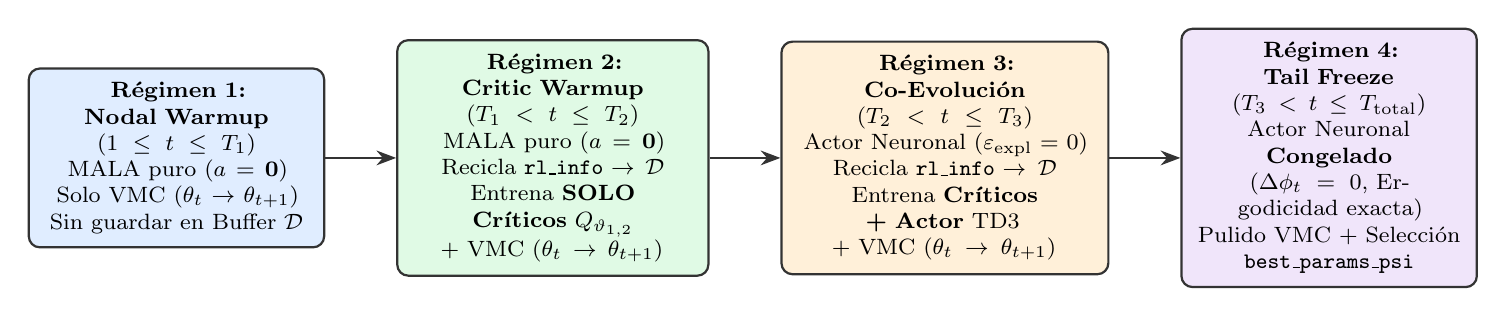
\begin{tikzpicture}[
    node distance=0.65cm and 0.9cm,
    box/.style={rectangle, rounded corners=4pt, draw=black!80, thick, align=center, font=\footnotesize, minimum height=0.95cm, inner sep=5pt},
    arrow/.style={-{Stealth[length=2.5mm]}, thick, draw=black!80}
]
\node[box, fill=phase1col, text width=3.4cm] (r1) {\textbf{R\'egimen 1: Nodal Warmup}\\($1 \le t \le T_1$)\\MALA puro ($a=\bm{0}$)\\Solo VMC ($\theta_t \to \theta_{t+1}$)\\Sin guardar en Buffer $\mathcal{D}$};
\node[box, fill=phase2col, text width=3.6cm, right=of r1] (r2) {\textbf{R\'egimen 2: Critic Warmup}\\($T_1 < t \le T_2$)\\MALA puro ($a=\bm{0}$)\\Recicla \texttt{rl\_info} $\to \mathcal{D}$\\Entrena \textbf{SOLO Cr\'iticos} $Q_{\vartheta_{1,2}}$\\+ VMC ($\theta_t \to \theta_{t+1}$)};
\node[box, fill=phase3col, text width=3.8cm, right=of r2] (r3) {\textbf{R\'egimen 3: Co-Evoluci\'on}\\($T_2 < t \le T_3$)\\Actor Neuronal ($\varepsilon_{\mathrm{expl}}=0$)\\Recicla \texttt{rl\_info} $\to \mathcal{D}$\\Entrena \textbf{Cr\'iticos + Actor} TD3\\+ VMC ($\theta_t \to \theta_{t+1}$)};
\node[box, fill=phase4col, text width=3.4cm, right=of r3] (r4) {\textbf{R\'egimen 4: Tail Freeze}\\($T_3 < t \le T_{\mathrm{total}}$)\\Actor Neuronal \textbf{Congelado}\\($\Delta\phi_t = 0$, Ergodicidad exacta)\\Pulido VMC + Selecci\'on\\\texttt{best\_params\_psi}};

\draw[arrow] (r1) -- (r2);
\draw[arrow] (r2) -- (r3);
\draw[arrow] (r3) -- (r4);
\end{tikzpicture}
\caption{Arquitectura secuencial de los 4 Reg\'imenes del Pipeline 4 (\texttt{OnlineCoupledTrainer1D}). En todos los pasos $t=1,\dots,T_{\mathrm{total}}$ se optimiza $\Psi_{\theta_t}$ por VMC sin ejecutar un solo barrido MCMC redundante.}
\label{fig:pipeline4_diagram}
\end{figure}

---

\section{Marco Te\'orico y Ecuaciones Gobernantes}

\subsection{Hamiltoniano F\'isico y Ansatz Variacional Slater-Jastrow-Backflow (SJB)}

El sistema f\'isico de $N = N_\uparrow + N_\downarrow$ electrones en un punto cu\'antico arm\'onico unidimensional con interacci\'on de Coulomb suavizada (\texttt{Harmonic1DHamiltonian} en \texttt{rl\_vmc/physics/harmonic\_1d.py}) est\'a gobernado por el Hamiltoniano:
\begin{equation}
\hat{H} = -\frac{1}{2}\sum_{i=1}^{N} \frac{\partial^2}{\partial x_i^2} + \frac{1}{2}\omega^2 \sum_{i=1}^{N} x_i^2 + \sum_{1 \le i < j \le N} \frac{g}{\sqrt{(x_i - x_j)^2 + a^2}}.
\label{eq:hamiltonian}
\end{equation}

La funci\'on de onda variacional $\Psi_\theta(X)$ (\texttt{SlaterJastrow1DAnsatz} o \texttt{MultiSlaterJastrowBackflow1DAnsatz} en \texttt{rl\_vmc/ansatze/ansatz\_1d.py}) se expresa en dominio logar\'itmico como:
\begin{equation}
\log |\Psi_\theta(X)| = \log \left| \sum_{k=1}^{M_{\mathrm{det}}} c_k \, \det\!\left[\phi_{k,a}^\uparrow(\tilde{x}_{i,\uparrow})\right]_{i,a=1}^{N_\uparrow} \det\!\left[\phi_{k,b}^\downarrow(\tilde{x}_{j,\downarrow})\right]_{j,b=1}^{N_\downarrow} \right| + J_\theta(X),
\label{eq:ansatz_sjb}
\end{equation}
donde la transformaci\'on de coordenadas de \textbf{Backflow} $\tilde{x}_i(X)$ desplaza las superficies nodales de acuerdo con la configuraci\'on instant\'anea de los dem\'as electrones:
\begin{equation}
\tilde{x}_i = x_i + \sum_{j \ne i} (x_i - x_j)\, e^{-(x_i - x_j)^2 / L_{\mathrm{env}}^2} \sum_{m=1}^{K_{\mathrm{bf}}} w_{m,\sigma_i\sigma_j} \exp\!\left(-\frac{(|x_i - x_j| - \mu_m)^2}{2w_{\mathrm{bf}}^2}\right),
\end{equation}
y el factor de correlaci\'on de \textbf{Jastrow-RBF} $J_\theta(X)$ modela la c\'uspide repulsiva electr\'on-electr\'on resuelta por canal de esp\'in ($\uparrow\uparrow / \downarrow\downarrow$ frente a $\uparrow\downarrow$).

\subsection{Energ\'ia Local y Estimador de Gradiente VMC con Recorte MAD (\texttt{vmc\_update\_step})}

Para cada configuraci\'on de caminante $X^{(b)} \in \mathbb{R}^{N \times 1}$ ($b = 1, \dots, B$), la energ\'ia local $E_L(X) = \Psi_\theta(X)^{-1}\hat{H}\Psi_\theta(X)$ se calcula exactamente como:
\begin{equation}
E_L(X) = \underbrace{-\frac{1}{2}\sum_{i=1}^{N} \left[ \frac{\partial^2 \log|\Psi_\theta(X)|}{\partial x_i^2} + \left(\frac{\partial \log|\Psi_\theta(X)|}{\partial x_i}\right)^2 \right]}_{T_{\mathrm{loc}}(X)} + \underbrace{\frac{1}{2}\omega^2 \sum_{i=1}^{N} x_i^2 + \sum_{1 \le i < j \le N} \frac{g}{\sqrt{(x_i - x_j)^2 + a^2}}}_{V_{\mathrm{loc}}(X)}.
\label{eq:local_energy}
\end{equation}

En las proximidades de los nodos ($\Psi_\theta(X) = 0$), $E_L(X)$ exhibe colas de ley de potencias. Para estabilizar el gradiente variacional sin introducir sesgo asint\'otico, \texttt{vmc\_update\_step} (\texttt{rl\_vmc/trainers/runner\_1d.py}) aplica un filtro robusto basado en la mediana $m_t$ y la desviaci\'on absoluta mediana ($\mathrm{MAD}_t$):
\begin{equation}
m_t = \mathrm{median}_b\!\big(E_L(X_t^{(b)})\big), \qquad \mathrm{MAD}_t = \mathrm{median}_b\!\big(|E_L(X_t^{(b)}) - m_t|\big) + 10^{-8},
\end{equation}
\begin{equation}
\tilde{E}_L(X_t^{(b)}) = \mathrm{clip}\!\Big(E_L(X_t^{(b)}),\; m_t - k_\sigma \mathrm{MAD}_t,\; m_t + k_\sigma \mathrm{MAD}_t\Big), \qquad \bar{E}_t = \frac{1}{B}\sum_{b=1}^{B} \tilde{E}_L(X_t^{(b)}).
\end{equation}
El gradiente variacional respecto a los par\'ametros $\theta$ se obtiene mediante diferenciaci\'on autom\'atica sobre la funci\'on de p\'erdida sustituta:
\begin{equation}
\mathcal{L}_{\mathrm{VMC}}(\theta) = \frac{2}{B}\sum_{b=1}^{B} \mathrm{stop\_gradient}\!\Big(\tilde{E}_L(X_t^{(b)}) - \bar{E}_t\Big) \log|\Psi_\theta(X_t^{(b)})|, \qquad \bm{g}_t^\theta = \nabla_\theta \mathcal{L}_{\mathrm{VMC}}(\theta_t),
\label{eq:vmc_grad}
\end{equation}
aplicando recorte por norma global ($\|\bm{g}_t^\theta\|_2 \le G_{\max}$) y actualizaci\'on con Adam (\texttt{optax.adam}) bajo un planificador cosenoidal con calentamiento lineal.

\subsection{Propuesta Neuronal Residual-MALA con DeepSets Equivariantes}

El kernel de propuesta neuronal \texttt{DeepSetNeuralProposal1D} (\texttt{rl\_vmc/proposals/proposals\_1d.py}) construye para cada electr\'on $i \in \{1,\dots,N\}$ el vector de estado $s_t^{(b,i)} \in \mathbb{R}^{d_s}$ mediante \texttt{build\_particle\_features\_1d}:
\begin{equation}
s_t^{(b,i)} = \Big[\, \underbrace{x_i,\; x_i - \bar{x}^{(b)},\; \tanh\!\big(F_{Q,i}(X^{(b)})/s_F\big),\; \sigma_i}_{\text{Local (4 dims)}},\;\; \underbrace{\tfrac{N}{s_N},\; \tfrac{N_\uparrow}{N},\; \tanh(\omega),\; \tanh(g),\; \tanh(a)}_{\text{Global (5 dims)}},\;\; \underbrace{\mathcal{S}_{\mathrm{same}}^{(b,i)}}_{\text{Vecinos }\sigma_j=\sigma_i},\;\; \underbrace{\mathcal{S}_{\mathrm{opp}}^{(b,i)}}_{\text{Vecinos }\sigma_j\ne\sigma_i} \,\Big],
\end{equation}
donde $F_{Q,i}(X) = \partial_{x_i}\log|\Psi_\theta(X)|$ es la deriva de Langevin y $\mathcal{S}_{\mathrm{same}}, \mathcal{S}_{\mathrm{opp}}$ contienen las ternas ordenadas por distancia $(|x_i - x_j|/s_r,\, \mathrm{sign}(x_i - x_j),\, \mathbb{I}_{\mathrm{activo}})$. La red \texttt{FlaxTD3Actor} aplica encoders MLP compartidos con activaci\'on SiLU y \textit{sum-pooling} sobre los vecinos de cada canal de esp\'in, produciendo la acci\'on acotada $a_t^{(b,i)} = (a_{\mu,i}, a_{\sigma,i}) \in (-1, 1) \times (-s_\sigma, s_\sigma)$.

En el modo \texttt{residual\_mala} (\texttt{ResidualMALAPolicy1D.compute\_distribution}), la propuesta gaussiana hacia adelante $X' \sim q_{\phi_t}(\cdot \mid X) = \mathcal{N}(\bm{\mu}_{\phi_t}(X), \mathrm{diag}(\bm{\sigma}_{\phi_t}^2(X)))$ toma la forma:
\begin{align}
\mu_{\phi_t, i}(X) &= x_i + \tau \, \mathrm{clip}\!\big(\nabla_{x_i}\log|\Psi_{\theta_t}(X)|, -D_{\max}, D_{\max}\big) + A \, g_{\mathrm{spat}}(x_i)\, a_{\mu, i}\!\big(s_t^{(i)}\big), \label{eq:res_mala_mu} \\
\sigma_{\phi_t, i}(X) &= \sqrt{2\tau} \, \exp\!\Big(\mathrm{clip}\!\big(g_{\mathrm{spat}}(x_i)\, a_{\sigma, i}\!\big(s_t^{(i)}\big),\; c_{\min},\; c_{\max}\big)\Big), \label{eq:res_mala_sigma}
\end{align}
donde $g_{\mathrm{spat}}(x_i) = (1 + x_i^2 / R_{\mathrm{gate}}^2)^{-1/2}$ es el factor de contenci\'on espacial (Ecuaci\'on 30 de Wang et al., 2024). Como las capas de salida de \texttt{FlaxTD3Actor} se inicializan exactamente en cero (\texttt{nn.initializers.zeros}), cuando $\phi = \phi_0$ se tiene $a_{\mu,i} = 0$ y $a_{\sigma,i} = 0$, reduciendo las Ecuaciones \eqref{eq:res_mala_mu}--\eqref{eq:res_mala_sigma} de forma exacta al algoritmo MALA cl\'asico.

\subsection{Invariancia por Metropolis-Hastings y Recompensa CDLB Fuera de Estacionariedad}

Toda propuesta $X'$ es filtrada por el paso de aceptaci\'on-rechazo de Metropolis-Hastings en \texttt{MHSampler1D.step}:
\begin{equation}
\alpha_t(X, X') = \min\!\left\{ 1,\; \frac{|\Psi_{\theta_t}(X')|^2 \, q_{\phi_t}(X \mid X')}{|\Psi_{\theta_t}(X)|^2 \, q_{\phi_t}(X' \mid X)} \right\}.
\label{eq:mh_alpha}
\end{equation}
Siguiendo el \textbf{Remark 3 de Wang et al.\ (2024)} (\texttt{2405.13574v1-2.pdf}, p\'ag.\ 7), al evolucionar la cadena de Markov con la pol\'itica determinista ($\varepsilon_{\mathrm{expl}} = 0$), el kernel de transici\'on $K_{\theta_t, \phi_t}$ preserva exactamente la distribuci\'on instant\'anea $|\Psi_{\theta_t}(X)|^2$ en cada paso $t$, garantizando que el estimador del gradiente variacional \eqref{eq:vmc_grad} sea insesgado.

Asimismo, siguiendo a \textbf{Wang et al.\ (2025)} (\texttt{2507.00671v1.pdf}, Secciones 2.2--2.3), cuando la cadena o la densidad objetivo $|\Psi_{\theta_t}|^2$ evolucionan en el tiempo, el criterio \textbf{CDLB} (\textit{Contrastive Divergence Lower Bound}, implementado en \texttt{compute\_cdlb\_reward}) maximiza la reducci\'on en un paso de la divergencia KL $D_{\mathrm{KL}}(P_t \parallel |\Psi_{\theta_t}|^2) - D_{\mathrm{KL}}(P_{t+1} \parallel |\Psi_{\theta_t}|^2)$ mediante la recompensa:
\begin{equation}
r_t^{\mathrm{CDLB}}(X, X') = \lambda_{\mathrm{pen}} \Big[ \underbrace{\mathrm{clip}\!\big(2\alpha_t (\log|\Psi_{\theta_t}(X')| - \log|\Psi_{\theta_t}(X)|), -5, 5\big)}_{r_{\mathrm{exploit}}} + \underbrace{\big(-\alpha_t \log\alpha_t - (1-\alpha_t)\log(1-\alpha_t)\big)}_{r_{\mathrm{entropy}}} \Big] + \underbrace{\alpha_t \log\!\left(1 + \frac{\min(\|X'-X\|_1/N, d_{\max})^2}{\epsilon_r}\right)}_{r_{\mathrm{explore}}}.
\label{eq:cdlb_reward}
\end{equation}

\subsection{Aproximaci\'on Estoc\'astica en Dos Escalas de Tiempo, Reward Centering y Ergodicidad}

Bas\'andonos en la teor\'ia de aproximaci\'on estoc\'astica en dos escalas de tiempo (Murphy, 2025, \texttt{2412.05265v2.pdf}, Secciones 2.5.2.7 y 4.3.1; Yang et al., 2018, \texttt{1802.05438v5.pdf}, Teoremas 1 y 2) y en el Algoritmo 2 de Wang et al.\ (2025) (\texttt{2507.00671v1.pdf}, Ap\'endice D.1), el entrenador \texttt{TD3Learner1D} incorpora:

\begin{enumerate}
\item \textbf{Reward Centering ($\bar{R}_k$):} En tareas continuas de MCMC donde la energ\'ia y la escala media de recompensa se desplazan conforme $\Psi_{\theta_t}$ converge, restamos la media m\'ovil exponencial $\bar{R}_k = (1 - \eta_R)\bar{R}_{k-1} + \eta_R \langle r \rangle_{\mathcal{B}}$ en el objetivo TD de los Cr\'iticos gemelos:
\begin{equation}
y_i = \big(r_i - \bar{R}_k\big) + \gamma_{\mathrm{TD3}} \min_{j=1,2} Q_{\vartheta'_j}\!\Big(s'_i,\; \mathrm{clip}\big(\pi_{\phi'}(s'_i) + \mathrm{clip}(\epsilon, -c, c), -1, 1\big)\Big).
\label{eq:bellman_centered}
\end{equation}
\item \textbf{Actualizaci\'on de Polyak desacoplada durante el Calentamiento del Cr\'itico (R\'egimen 2):} En \texttt{TD3Learner1D.update\_step(key, allow\_actor\_update)}, cuando \texttt{allow\_actor\_update=False} (R\'egimen 2), los par\'ametros del Actor $\phi$ y del Actor objetivo $\phi'$ permanecen congelados en cero ($a=\bm{0}$), pero tanto los Cr\'iticos online $(\vartheta_1, \vartheta_2)$ como los Cr\'iticos objetivo $(\vartheta'_1, \vartheta'_2)$ se actualizan, permitiendo que $Q_{\vartheta_{1,2}}(s, a=\bm{0})$ converja suavemente al valor real de la pol\'itica base MALA antes de habilitar los gradientes del Actor en el R\'egimen 3.
\item \textbf{Teorema de Ergodicidad (Contenci\'on + Adaptaci\'on Decreciente, Teorema 2 de Wang et al., 2024):} La acotaci\'on $\tanh$ de las acciones junto con $g_{\mathrm{spat}}(x_i)$ garantiza la condici\'on de \textit{Containment}, mientras que el \textbf{R\'egimen 4 (\texttt{TailFreeze})}, en el cual se fijan $(\phi_t, \vartheta_t) \equiv (\phi_{T_3}, \vartheta_{T_3})$ ($\|\phi_{t+1} - \phi_t\| = 0$) durante los \'ultimos $N_{\mathrm{freeze}}$ pasos de VMC, garantiza estrictamente la condici\'on de \textit{Diminishing Adaptation} y la estacionariedad exacta de la cadena al seleccionar \texttt{best\_params\_psi}.
\end{enumerate}

---

\section{Arquitectura de Software y Especificaci\'on de Clases y Funciones}

Siguiendo el principio de m\'axima reutilizaci\'on modular, el Pipeline 4 reutiliza \'integramente \texttt{Harmonic1DHamiltonian}, \texttt{build\_ansatz\_1d}, \texttt{DeepSetNeuralProposal1D}, \texttt{MHSampler1D}, \texttt{compute\_rl\_reward} y \texttt{vmc\_update\_step}, introduciendo \'unicamente la clase dedicada \texttt{OnlineCoupledTrainer1D} y las extensiones necesarias en \texttt{TD3Learner1D} y \texttt{Experiment1DConfig}:

\begin{table}[H]
\centering
\caption{Mapeo exacto entre componentes algor\'itmicos del Pipeline 4 y funciones/clases del c\'odigo.}
\label{tab:code_mapping}
\begin{adjustbox}{max width=\textwidth}
\begin{tabular}{llll}
\toprule
\textbf{Archivo} & \textbf{Clase / Funci\'on} & \textbf{Rol en Pipeline 4 (\texttt{online\_coupled})} & \textbf{Ecuaciones} \\
\midrule
\texttt{rl\_vmc/trainers/online\_coupled\_trainer\_1d.py} & \texttt{OnlineCoupledTrainer1D.run} & Bucle maestro de los 4 reg\'imenes, cronometraje crudo y acoplamiento paso a paso & Fig.\ \ref{fig:pipeline4_diagram} \\
\texttt{rl\_vmc/trainers/online\_coupled\_trainer\_1d.py} & \texttt{get\_phase\_id\_and\_label} & Clasificaci\'on del paso $t$ en R1 (\texttt{NodalWarmup}), R2 (\texttt{CriticWarmup}), R3 (\texttt{CoEvolution}), R4 (\texttt{TailFreeze}) & $T_1, T_2, T_3$ \\
\texttt{rl\_vmc/samplers/mh\_sampler\_1d.py} & \texttt{MHSampler1D.step} & Propuesta Residual-MALA, filtro MH exacto y generaci\'on gratuita de \texttt{rl\_info} & Ecs.\ \eqref{eq:res_mala_mu}--\eqref{eq:mh_alpha} \\
\texttt{rl\_vmc/rl/rewards.py} & \texttt{compute\_rl\_reward} / \texttt{compute\_cdlb\_reward} & C\'alculo vectorizado de $r_t^{\mathrm{CDLB}}$ ($r_{\mathrm{exploit}}, r_{\mathrm{entropy}}, r_{\mathrm{explore}}$) desde \texttt{rl\_info} & Ec.\ \eqref{eq:cdlb_reward} \\
\texttt{rl\_vmc/rl/learners\_1d.py} & \texttt{TD3Learner1D.push\_transitions} & Submuestreo aleatorio de $M=\text{\texttt{online\_walkers\_to\_store}}$ caminantes e inserci\'on al buffer FIFO & Ventana FIFO \\
\texttt{rl\_vmc/rl/learners\_1d.py} & \texttt{TD3Learner1D.update\_step} & Paso TD3 con \texttt{allow\_actor\_update} (False en R2, True en R3) y \textit{Reward Centering} $\bar{R}_k$ & Ec.\ \eqref{eq:bellman_centered} \\
\texttt{rl\_vmc/trainers/runner\_1d.py} & \texttt{vmc\_update\_step} & Energ\'ia local por bloques, recorte MAD y paso de gradiente Adam sobre $\Psi_\theta$ & Ecs.\ \eqref{eq:local_energy}--\eqref{eq:vmc_grad} \\
\texttt{rl\_vmc/postprocess/plotter.py} & \texttt{run\_postprocessing\_pipeline} & Generaci\'on de figuras PNG/PDF y exportaci\'on de CSVs crudos de cada figura a \texttt{results\_csv/} & Post-proceso \\
\bottomrule
\end{tabular}
\end{adjustbox}
\end{table}

---

\section{An\'alisis de los 4 Casos de Ablaci\'on y B\'usqueda de Hiperpar\'ametros}

El orquestador \texttt{run\_pipeline4\_param\_search.sh} eval\'ua de forma controlada tanto las dos baselines previas (\texttt{VMC\_MALA} y \texttt{P3\_BlockCoupled}) como los \textbf{4 Casos de Ablaci\'on} de los reg\'imenes del Pipeline 4 sobre un mismo sistema f\'isico:

\begin{table}[H]
\centering
\caption{Casos de ablaci\'on de reg\'imenes implementados en \texttt{run\_pipeline4\_param\_search.sh}.}
\label{tab:ablation_cases}
\begin{adjustbox}{max width=\textwidth}
\begin{tabular}{lllll}
\toprule
\textbf{Identificador del Modelo} & \textbf{Configuraci\'on $(N_{\mathrm{nodal}}, N_{\mathrm{critic}}, N_{\mathrm{freeze}})$} & \textbf{Comportamiento Algor\'itmico} & \textbf{Hip\'otesis / Fen\'omeno Evaluado} \\
\midrule
\texttt{01\_Baseline\_VMC\_MALA} & \texttt{train\_mode=vmc\_only} & VMC est\'andar con MALA puro ($a=\bm{0}$) todo el tiempo & Referencia base sin aprendizaje por refuerzo \\
\texttt{02\_Baseline\_P3\_BlockCoupled} & \texttt{train\_mode=coupled} (6 ciclos) & Bloques alternados VMC y RL con sweeps extra & Costo de c\'omputo extra y desfase entre bloques \\
\texttt{03\_P4\_RegimeA\_ColdStart} & $(0,\; 0,\; 0)$ & Activa y entrena Actor + Cr\'itico desde el paso $t=1$ & Efecto del transiente nodal inicial y cr\'itico aleatorio \\
\texttt{04\_P4\_RegimeB\_BlindWarmup} & $(2N_{\mathrm{warm}},\; 0,\; N_{\mathrm{freeze}})$ & Warmup nodal con MALA sin pre-entrenar Cr\'itico & Salto transitorio en $t=T_1+1$ por cr\'itico no inicializado \\
\texttt{05\_P4\_RegimeC\_NoTailFreeze} & $(N_{\mathrm{warm}},\; N_{\mathrm{warm}},\; 0)$ & Warmup nodal + Pre-entrenamiento de Cr\'itico, sin R4 & Impacto de omitir la cola de adaptaci\'on decreciente \\
\texttt{06+ \_P4\_Full4R\_*} & $(N_{\mathrm{nodal}},\; N_{\mathrm{critic}},\; N_{\mathrm{freeze}}) > 0$ & \textbf{Pipeline 4 Completo (4 Reg\'imenes)} & Estabilidad del Cr\'itico desde $a=\bm{0}$ + ergodicidad final \\
\bottomrule
\end{tabular}
\end{adjustbox}
\end{table}

---

\section{Gu\'ia de Ejecuci\'on en Ayler (3 GPUs) y Caracter\'isticas QOL}

\subsection{Caracter\'isticas de Calidad de Vida (QOL) Integradas}

Ambos orquestadores nuevos (\texttt{run\_pipeline4\_param\_search.sh} y \texttt{run\_pipeline4\_benchmark.sh}, as\'i como \texttt{run\_production\_benchmark\_3pipelines.sh}) implementan:
\begin{itemize}
\item \textbf{Timestamps y Tiempo de C\'omputo Crudo (Raw Compute Time):} Cada log individual y el log maestro registran marcas de tiempo \texttt{YYYY-MM-DD HH:MM:SS}, el tiempo crudo en segundos (\texttt{train\_wall\_time\_sec}, \texttt{phase\_1\_sec..phase\_4\_sec}, \texttt{wall\_time\_sec}, \texttt{total\_run\_wall\_time\_sec}) y formato legible \texttt{HHh MMm SSs}.
\item \textbf{Par\'ametros Completos en Logs Individuales y Resumen en el Log Maestro:} Al iniciar cada corrida, \texttt{runner\_1d.py} imprime el JSON completo de configuraci\'on en el log individual; al finalizar el script maestro, se imprime una tabla consolidada y ordenada con todas las m\'etricas f\'isicas y tiempos de todas las corridas.
\item \textbf{CSVs de Todas las Figuras Guardados Aparte:} Todos los CSVs de m\'etricas, historiales de entrenamiento y datos crudos de cada figura (\texttt{figure\_data\_acf\_energy\_*.csv}, \texttt{figure\_data\_kl\_convergence\_*.csv}, \texttt{figure\_data\_walker\_traces\_*.csv}, \texttt{figure\_data\_all\_models\_summary.csv}, \texttt{observables\_*.csv}) se copian autom\'aticamente a \texttt{<CARPETA\_SALIDA>/results\_csv/}.
\item \textbf{Figuras en PNG por Defecto con Opci\'on PDF de Alto DPI y \texttt{--postprocess-only}:} Por defecto se exportan en \texttt{.png} a $300\text{ DPI}$ para ahorrar disco; pasando \texttt{--postprocess-only --pdf --dpi 600} (o \texttt{--both-formats}) se recompilan en CPU en formato vectorial PDF de alta resoluci\'on sin tocar las GPUs.
\item \textbf{Gesti\'on Inteligente de Memoria GPU y Sistema de Colas Multi-Trabajo por GPU:} El despachador detecta las GPUs disponibles (o recibe \texttt{--gpus "0 1 2"}), permite colocar m\'ultiples trabajos por GPU (\texttt{--jobs-per-gpu 2}, ideal para las GPUs de Ayler) y ajusta autom\'aticamente \texttt{XLA\_PYTHON\_CLIENT\_MEM\_FRACTION} ($0.75$ para $1$ job/GPU, $0.42$ para $2$ jobs/GPU, $0.28$ para $3$ jobs/GPU) con \texttt{XLA\_PYTHON\_CLIENT\_PREALLOCATE=false}.
\end{itemize}

\subsection{Comandos Exactos para Correr en Ayler}

\begin{lstlisting}[language=bash]
# 0. Actualizar repositorio y activar entorno en Ayler
cd ~/RL-VMC-main
git pull origin main
conda activate jax-gpu

# 1. PIPELINE DE BUSQUEDA DE HIPERPARAMETROS Y ABLACION DE 4 REGIMENES
#    Por defecto corre sobre N=4 (g=4.0) y N=6 (g=1.0) usando las 3 GPUs con 2 trabajos/GPU (6 en paralelo):
nohup ./run_pipeline4_param_search.sh \
    --systems "N4:4.0 N6:1.0" \
    --preset fast \
    --gpus "0 1 2" \
    --jobs-per-gpu 2 \
    > master_p4_search_ayler.log 2>&1 &

#    Para correr la busqueda sobre UN SOLO sistema en concreto (ej. N=4, g=4.0):
nohup ./run_pipeline4_param_search.sh \
    --systems "N4:4.0" \
    --preset fast \
    --gpus "0 1 2" \
    --jobs-per-gpu 2 \
    results_p4_search_N4_g4.0 > master_p4_search_N4.log 2>&1 &

# 2. PIPELINE DE BENCHMARK MULTI-SISTEMA (N, g) PARA PIPELINE 4
#    Por defecto recorre el grupo piloto de 3 sistemas (N4:2.0, N4:4.0, N6:1.0):
nohup ./run_pipeline4_benchmark.sh \
    --gpus "0 1 2" \
    --jobs-per-gpu 2 \
    > master_p4_pilot3_ayler.log 2>&1 &

#    Para comparar directamente Pipeline 3 (bloques) vs Pipeline 4 (online 4 regimenes):
nohup ./run_pipeline4_benchmark.sh \
    --with-p3 \
    --systems "N4:2.0 N4:4.0 N6:1.0" \
    --gpus "0 1 2" \
    --jobs-per-gpu 2 \
    results_p3_vs_p4_benchmark > master_p3_vs_p4.log 2>&1 &

#    Para recorrer toda la grilla completa (N in {2,4,6,10}, g in {0.1..8.0}):
nohup ./run_pipeline4_benchmark.sh \
    --full-grid \
    --gpus "0 1 2" \
    --jobs-per-gpu 2 \
    results_p4_full_production > master_p4_full_ayler.log 2>&1 &

# 3. POST-PROCESAMIENTO UNICAMENTE Y COMPILACION EN PDF A 600 DPI
./run_pipeline4_param_search.sh results_pipeline4_param_search --postprocess-only --pdf --dpi 600
./run_pipeline4_benchmark.sh results_pipeline4_benchmark --postprocess-only --pdf --dpi 600
\end{lstlisting}

\begin{thebibliography}{9}
\bibitem{Wang2024}
Z.\ Wang, Y.\ Chen, M.\ Kanagawa, C.\ J.\ Oates, \textit{Reinforcement Learning for Adaptive MCMC}, arXiv:2405.13574v1 (2024).

\bibitem{Wang2025}
Z.\ Wang, M.\ Fisher, M.\ Kanagawa, Y.\ Chen, C.\ J.\ Oates, \textit{Harnessing the Power of Reinforcement Learning for Adaptive MCMC}, arXiv:2507.00671v1 (2025).

\bibitem{Murphy2025}
K.\ P.\ Murphy, \textit{Reinforcement Learning: A Comprehensive Overview}, arXiv:2412.05265v2 (2025).

\bibitem{Schulman2015}
J.\ Schulman, S.\ Levine, P.\ Moritz, M.\ I.\ Jordan, P.\ Abbeel, \textit{Trust Region Policy Optimization}, arXiv:1502.05477v5 (2015).

\bibitem{Yang2018}
Y.\ Yang, R.\ Luo, M.\ Li, M.\ Zhou, W.\ Zhang, J.\ Wang, \textit{Mean Field Multi-Agent Reinforcement Learning}, ICML / arXiv:1802.05438v5 (2018).

\bibitem{Kumar2024}
S.\ Kumar et al., \textit{Adaptive dynamics of Ising spins in one dimension leveraging Reinforcement Learning}, arXiv:2411.19602v1 (2024).
\end{thebibliography}

\end{document}
